\documentclass[a4paper,10pt]{article}

\usepackage{hyperref}
\usepackage{graphicx, float}
\usepackage[dutch]{babel}

\hypersetup{colorlinks=true, linkcolor=cyan}

%opening
\title{Plan van Aanpak - Gedistribueerde systemen 2010}
\author{Team 7 \\
Jan Laan - 5756529\\
Bas Vlaszaty - 5783445 \\
Saidou Diallo - 6215297\\
Ravish Gopal - }

\begin{document}

  \maketitle
  \newpage
  \section{Inleiding}
  Voor het college Gedistribueerde Systemem 2010 maken wij een chatserver. Deze server is onderdeel van een groep servers die samen een chat-netwerk vormen. De server moet rekening houden met meerdere andere servers en meerdere clients die eraan verbonden zijn. Ook heeft de server een continue verbinding met de \textit{control server}.
  
  \section{Implementatie}
  Als implementatietaal is gekozen voor Python. We zijn niet heel bekend met deze taal. Sommigen hebben wel wat in Python gedaan, sommigen helemaal niet. Dit is een mooie gelegenheid om een nieuwe taal te leren kennen. Daarnaast is Python een taal waarin je relatief snel kunt programmeren. Het is compact en zit vol met handige functies. Omdat het een ge\"interpreteerde taal is is het niet heel snel. Wij denken dat dit geen problemen gaat opleveren omdat de server niet zwaar belast gaat worden. Als dit wel het geval zou zijn is het handiger om voor een gecompileerde taal te kiezen.

  \section{Analyse}
  Het protocol is gebaseerd op een boomstructuur. Elke server kan maar 1 actieve connectie hebben met een andere server (wat dus de parent is) maar er kunnen meerdere servers verbinding met hem aangaan (children). Door deze opzet blijft het dus altijd een boom. Dit is belangrijk omdat een boom per definitie geen cykels bevat. Als er namelijk cykels van servers zouden ontstaan zou de mogelijkheid bestaan dat een bericht in die cykel rond blijft gaan en nooit bij zijn bestemming aankomt. Dit willen we natuurlijk voorkomen. Een groot deel van de commando’s is bedoelt om te zorgen dat die structuur van de servers intact blijft. Om dit alles in goede banen te leiden heeft elke server een database met daarin gegevens over de actieve verbindingen en de status van het netwerk. Elke server heeft dus 4 soorten verbindingen:
\begin{itemize}
\item 1 verbinding naar een parent
\item 1 verbinding naar de control server
\item Many verbindingen naar child servers
\item Many verbindingen naar clients
\end{itemize}

Qua type berichten zijn er 7 types. Client-server, server-client en server-server worden gebruikt voor het onderhoud van het netwerk en voor het versturen en bezorgen van de berichten van de ene client naar de andere. Controlserver-server en server-controlserver berichten worden gebruikt voor het toevoegen van een nieuwe server aan het al bestaande netwerk, of voor het hergroeperen van de servers als er een server wegvalt. Ook heb je controlserver-client en client-controlserver berichten maar daar hebben wij niet zo veel mee te maken aangezien we een server gaan programmeren. De totale verzameling aan beschikbare berichten lijkt me genoeg voor dit doel. Het is geen enorm uitgebreid protocol maar heeft wel de basic functionaliteit die je van een dergelijk protocol zou verwachten.

Ik zie echter ook wel problemen met het protocol zoals dat er nu is. Die problemen liggen vooral in de aard van consistentie van de informatie van de servers. Als er namelijk een server uitvalt hebben twee delen van het netwerk even geen verbinding meer met elkaar. Dit zal niet heel lang duren maar aangezien er na 30 seconden inactiviteit pas gepingt gaat worden is er in het slechtste geval 30 seconden geen verbinding tussen die 2 delen van het netwerk. Als in die tijd 2 personen met dezelfde naam zich aanmelden en een wordt toegewezen aan een server in het ene deel en de ander aan een server in het andere deel dan zijn er dus opeens 2 clients met dezelfde naam in het netwerk als dit weer gehergroepeerd wordt. Om dit te verhelpen lijkt het me het eenvoudigst om de authenticatie niet in de servers te doen maar om de control server dit te laten afhandelen. Dit betekend wel dat er een paar extra commando’s zullen moeten worden ingevoerd maar ik denk dat het de robuustheid van het systeem wel ten goede komt. Verder denk ik dat er sowieso nog beter gekeken moet worden naar scenario’s waarin een server uit de boom wegvalt. Dat zijn volgens mij namelijk de momenten waarop in dit systeem allerlei problemen ontstaan omdat je opeens twee losse netwerken hebt en consistentie van de informatie niet meer gegarandeert kan worden.

Al met al is het protocol dus basic, en het “serves the purpose” in dit geval. Ik zou er echter geen commercieel systeem op baseren. Daarvoor is het gewoon niet solide genoeg.

  \section{Software}
  Onze software zal worden opgedeeld in verschillende modules. Een duidelijk overzicht van de complete structuur is te zien in de onderstaande afbeelding.
  \begin{figure}[H]
    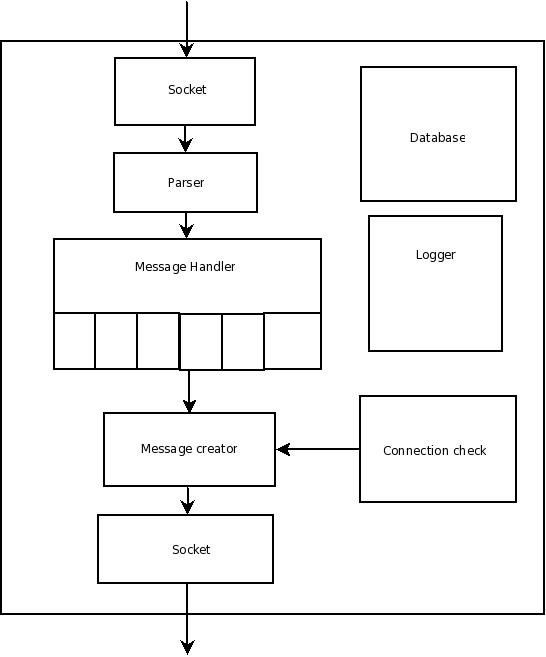
\includegraphics[width=0.9\textwidth]{dia1.jpg}
    \caption{Module-structuur}
  \end{figure}
  Er zijn twee soorten acties die de server onderneemt. Een is als de server een bericht binnenkrijgt. Daarop moet een actie ondernomen worden. De ander is de server die zelfstandig acties onderneemt, zoals pingen naar servers en clients. Uiteraard draaien beide in verschillende threads.
  
  \subsection{Inkomende verbindingen}
  De server luistert op een inkomende socket-verbinding. Als er iets binnenkomt wordt er een nieuw thread aangemaakt dat dat bericht gaat afhandelen. Het bericht wordt vervolgens eerst doorgestuurd naar een parser, die van het bericht iets leesbaars maakt. De leesbare opdracht wordt doorgestuurd naar de zogenaamde message handler. Deze handler bekijkt wat voor bericht er is binnengekomen. Op basis hiervan wordt het bericht verwerkt door een sub-module van de message handler. 
  
  \subsubsection{sub-modules van de handler}
  Deze sub-modules beslaan het meeste van onze code. Hier wordt de boodschap verwerkt en besloten wat voor actie wordt ondernomen. Bijvoorbeeld: Als een ping wordt ontvangen, besluit deze module dat er een pong wordt teruggestuurd naar de relevante client/server. Als er een tekstbericht binnenkomt, wordt dit geprobeerd te worden doorgestuurd naar de ontvanger. Als iets moet worden verstuurd neemt deze sub-module contact op met de message creator.

  \subsection{Uitgaande Verbindingen}
  De message creator ontvangt een leesbaar bericht en maakt er een message van volgens het gegeven protocol. Deze message wordt vervolgens naar de relevante socket(s) gestuurd.

  \subsection{Conenction check}
  De connection check is het actieve deel van de server. De rest wacht alleen op inkomende berichten, dit deel onderneemt zelfstandig actie. Alle servers/clients moeten regelmatig ge-pingd worden om te kijken of ze nog actief zijn. Dit gebeurt hier. Ping-boodschappen worden verzonden naar de message creator en vervolgens de socket.

  \subsection{database en logger}
  Als losse modules hebben we verder nog de database en de logger. Deze modules staan een beetje op zichzelf, en kunnen gebruikt worden door alle andere (sub)-modules. Deze 2 modules spreken voor zich, de database houdt gegevens bij zich zoals verbonden clients en servers, en de logger logt alle serverberichten naar relevante bestanden.


  \section{Werkverdeling}
  \begin{itemize}
    \item Verslag bijhouden: Jan
    \item Verder: Ieder kiest een module en maakt die.
  \end{itemize}
  Als eerst worden de volgende modules gemaakt:
\begin{itemize}
 \item Socket
  \item Database
  \item message parser/creator
\end{itemize}
  De rest is natuurlijk ook essentieel, maar komt daarna pas. Bovenstaande modules zijn de echte basis.

Om alles op een lijn te houden hebben we een git-repository voor versiebeheer.



  \section{Tijdsplanning}
  \begin{itemize}
    \item \textbf{Week 1 (31 Maart)}: Plan van aanpak, werkverdeling
    \item \textbf{Week 2 (7 April)}: Programmeren
    \item \textbf{Week 3 (14 April)}: Programmeren
    \item \textbf{Week 4 (21 April)}: Werkende versie af
    \item \textbf{Week 5 (28 April)}: Stabiele versie af
    \item \textbf{Week 6 (10 Mei)}: laatste tests, afronden verslag
    \item \textbf{Week 7 (12 Mei)}: gezamenlijke test

  \end{itemize}


\end{document}
